\documentclass{juliacon}

\setcounter{page}{1}

% \usepackage[skip=5pt]{caption}
\captionsetup{skip=10pt}
\usepackage{amsmath}
\usepackage[capitalize,nameinlink]{cleveref}
\usepackage[export]{adjustbox}
\graphicspath{{./graphics/}}

\crefname{listing}{Code}{Codes}

\definecolor{TolMutedBlue}{HTML}{332288}
\definecolor{TolMutedCyan}{HTML}{88CCEE}
\definecolor{TolMutedTeal}{HTML}{44AA99}
\definecolor{TolMutedGreen}{HTML}{117733}
\definecolor{TolMutedOlive}{HTML}{999933}
\definecolor{TolMutedSand}{HTML}{DDCC77}
\definecolor{TolMutedRose}{HTML}{CC6677}
\definecolor{TolMutedWine}{HTML}{882255}
\definecolor{TolMutedPurple}{HTML}{AA4499}

\hypersetup{%
    colorlinks=true,%
    urlcolor=TolMutedRose,%
    linkcolor=TolMutedBlue,%
    citecolor=TolMutedGreen%
}

\lstset{
  extendedchars=true,
  literate={∈}{{$\in$}}1 {⊆}{{$\subseteq$}}1 {≥}{{$\ge$}}1 {α}{{$\alpha$}}1 {ⁿ}{{{\textsuperscript{n}}}}1 {Rⁿ}{{{R\textsuperscript{n}}}}1
}

\def\F{\mathcal{F}}
\def\tp{\mathsf{T}}

% OPTIMIZATION
\DeclareMathOperator*{\argmin}{\arg\min}
\DeclareMathOperator*{\argmax}{\arg\max}
\DeclareMathOperator*{\minimize}{minimize}
\DeclareMathOperator*{\maximize}{maximize}
\DeclareMathOperator*{\minimum}{minimum}
\DeclareMathOperator*{\maximum}{maximum}
\DeclareMathOperator*{\subjectto}{subject\ to}
\DeclareMathOperator*{\st}{\text{s.t.}}
\DeclareMathOperator*{\feasible}{feasible}

% DERIVATIVES
\def\df{\nabla\!f}
\def\d{\mathrm{d}}
\def\ddt{\frac{\d}{\d t}}

% MATRIX CONSTRUCTORS
\newcommand{\mat}[1]{\begin{matrix}#1\end{matrix}}
\newcommand{\bmat}[1]{\begin{bmatrix}#1\end{bmatrix}}
\newcommand{\pmat}[1]{\begin{pmatrix}#1\end{pmatrix}}
\newcommand{\bmatl}[2]{\renewcommand{\arraystretch}{1.2}\left[\begin{array}{#1}#2\end{array}\right]}
\newcommand{\pmatl}[2]{\renewcommand{\arraystretch}{1.2}\left(\begin{array}{#1}#2\end{array}\right)}
\newcommand{\sbmat}[1]{\left[\begin{smallmatrix}#1\end{smallmatrix}\right]}
\newcommand{\spmat}[1]{\left(\begin{smallmatrix}#1\end{smallmatrix}\right)}


\begin{document}

% **************GENERATED FILE, DO NOT EDIT**************

\title{Automated Algorithm Analysis in Julia}

\author[1]{Sam Skinner}
\author[1]{Lam Ha}
\author[1]{Bryan Van Scoy}
\affil[1]{Miami University, Department of Electrical and Computer Engineering, Oxford, OH 45056, USA}

\keywords{Julia, Algorithm Analysis, Performance Estimation Problems, Control Theory}

\hypersetup{
pdftitle = {Automated Algorithm Analysis in Julia},
pdfsubject = {JuliaCon 2026 Proceedings},
pdfauthor = {Sam Skinner, Lam Ha, Bryan Van Scoy},
pdfkeywords = {Julia, Algorithm Analysis, Performance Estimation Problems, Control Theory},
}



\maketitle

\begin{abstract}

\href{https://github.com/vanscoy/AlgorithmAnalysis.jl/stable/}{\texttt{AlgorithmAnalysis.jl}} is a Julia package for the automated analysis of algorithms. The package provides a generic way to analyze algorithms in a systematic manner in the Julia programming language. Algorithm analysis seeks to find a mathematically proven guarantee of an algorithm's performance over a class of problems. AlgorithmAnalysis.jl includes both the performance estimation (PEP) and control theoretic methodologies to analysis.

\end{abstract}

\section{Introduction}


\href{https://github.com/vanscoy/AlgorithmAnalysis.jl/stable/}{\texttt{AlgorithmAnalysis.jl}} is a Julia package for the automated analysis of algorithms. The package provides a generic way to analyze algorithms in a systematic manner in the Julia programming language. Algorithm analysis seeks to find a mathematically proven guarantee of an algorithm's performance over a class of problems. AlgorithmAnalysis.jl includes both the performance estimation (PEP) and control theoretic methodologies to analysis.

Our package enables users to write optimization algorithms using simple syntax that resembles the mathematical algorithm structure, as illustrated in \cref{code:label}.

\begin{lstlisting}[
    language = Julia,
    % numbers = left,
    label = {code:label}, 
    caption = {Example Code Block.}
]
using AlgorithmAnalysis
m, L = 1, 10
α = 2 / (L + m)
@algorithm begin
    f = DifferentiableFunctional{Rⁿ}()
    xs = first_order_stationary_point(f)
    f ∈ SmoothStronglyConvex(m, L)
    x1 = x0 - α * f'(x0)
    x0 => x1
    performance = (x0 - xs)^2
end

# compute the worst-case convergence rate
rate(performance)
\end{lstlisting}

The automated analysis methodology has lead to the discovery of new algorithms and insights into existing algorithms. For example, the performance estimation problem (PEP) methodology has been used to analyze first-order optimization methods, leading to the discovery of new algorithms with improved convergence rates~\cite{pep}. The control theoretic analysis methodology has been used to analyze the stability and robustness of optimization algorithms, leading to the development of new algorithms that are more robust to noise and uncertainty.


\begin{figure}[t]
\centerline{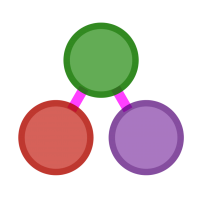
\includegraphics[width=4cm]{juliagraphs.png}}
\caption{This is example of the image in a column.}
	\label{fig:sample_figure}
\end{figure}

The figure \ref{fig:sample_figure} is taken from the JuliaGraphs
organization \footnote{https://github.com/JuliaGraphs}.

\section{Algorithm Analysis Methodologies}

Mathematically, optimization problems are modeled as minimizing a function subject to constraints. The automated analysis methodology applies to black-box algorithms, which obtain information about the objective function only through queries to an oracle that returns information about the queried point~\cite{nemirovski-yudin,nesterov-book}. %A first-order algorithm, for instance, uses the gradient oracle $\O_f(y) = \df(y)$.
The main idea is to study the properties of an algorithm applied to an optimization problem in a systematic way as illustrated in Figure~\ref{fig:overview}.

\begin{figure*}[t]
    \centering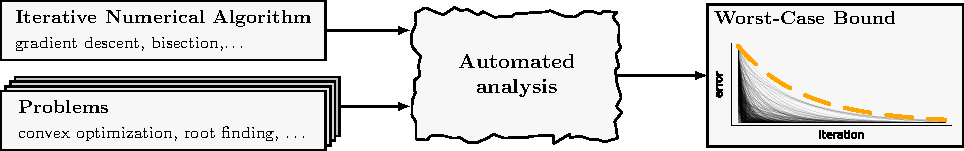
\includegraphics{overview}
    \caption{Overview of the automated algorithm analysis methodology. The automated analysis procedure solves a convex optimization problem to produce a convergence result.}
	\label{fig:overview}
\end{figure*}

There are two main approaches to automated algorithm analysis: the \textit{performance estimation problem} (PEP) approach from the optimization community and \textit{integral quadratic constraints} (IQCs) from the control community.

The PEP approach formulates the automated analysis as the problem of finding the sequence of iterates and the optimization problem for which a given algorithm attains its worst-case behavior in terms of a specified measure of performance over some finite number of iterations~\cite{drori-teboulle}. While this optimization problem involves searching over an infinite-dimensional class of functions, it can be convexified by replacing the search over the function itself with constraints on the iterates such that there exists some function in the class that interpolates the points, along with a large-scale asumption on the dimension of the underlying domain of the optimization problem~\cite{pep}. While the PEP approach constructs provably tight bounds on the iterates of the algorithm, it can do so only over finite time horizons. Furthermore, the complexity of the analysis scales with the number of iterations, so the analysis is only computationally tractable for up to a few hundred iterations.

In contrast, the IQC approach interprets an optimization algorithm as a dynamical system~\cite{lessard16}. Similar to the PEP approach, the ``uncertainty'' (such as the gradient of the objective function for first-order methods) is replaced by constraints between its inputs and outputs\footnote{The term \textit{integral quadratic constraint} comes from the fact that these constraints are often sums of quadratic forms, and the sums become integrals for continuous-time systems.}. These constraints are then used to search for a parameterized Lyapunov function whose existence is a certificate of convergence~\cite{taylor2018lyapunov}. This approach solves small semidefinite programs to produce bounds on the iterates of the algorithm that hold over any number of iterations. These bounds are tight in that, if a Lyapunov function of the parameterized form exists, this technique will find it~\cite{taylor2018lyapunov}. But there is in general no guarantee of such systems having a Lyapunov function of a particular form, so in general the convergence bounds may not be tight.

These approaches have been applied to a variety of algorithm forms such as fixed-step first-order methods~\cite{pep}, Nesterov's accelerated method~\cite{hu-lessard2017}, the alternating direction method of multipliers (ADMM)~\cite{admm,iqcadmm_ICML}, Markov jump linear systems~\cite{hu-syed2019}, inexact gradient and Newton methods~\cite{deklerk-glineur-taylor2020}, and decentralized methods~\cite{colla-hendrickx2023} among others.

While the convergence properties of an algorithm depend on the specific objective function $f$, algorithms are typically designed and analyzed for an entire class of functions $\F$. In this case, the goal may be to characterize the \textit{worst-case} performance of the algorithm over any objective function in the class~\cite{rmm}, or to characterize the distribution of the performance over all problems in the class (such as \textit{average-case} performance~\cite{robey-chamon-pappas-hassani2022}).

We now describe the main ideas behind the PEP and IQC approaches to worst-case automated algorithm analysis on the unconstrained optimization problem of minimizing an objective function $f$ in a class $\F$ of (differentiable) functions.

\subsection{Performance Estimation}

A performance estimation problem (PEP) is an optimization problem whose solution characterizes the exact worst-case convergence properties of a black-box algorithm over a finite number of iterations~\cite{pep-original,pep}. Given an oracle $O_f$ and initial point $y_0$, a black-box method $M$ constructs a sequence of points $y_1,y_2,\ldots$ as follows:
\begin{align*}
  y_1 &= M_0(y_0,O_f(y_0)), \\
  y_2 &= M_1(y_0,O_f(y_0),O_f(u_1)), \\
    &\ \, \vdots \\
  y_{k+1} &= M_k(y_0,O_f(y_0),\ldots,O_f(y_k)).
\end{align*}
At iteration $k$, the next iterate $y_{k+1}$ is constructed from the initial condition $y_0$ and the oracle applied to all the previous iterates, $O_f(y_0),\ldots,O_f(y_k)$. Given a function class $\F$, a black-box algorithm $M$, and an initial point $y_0$, a typical PEP has the form
\begin{align*}
  \maximize \quad & \text{performance of algorithm $M$ with oracle $O_f$ over $N$ iterations} \\
  \text{subject to} \quad & f\in\F
\end{align*}
where the variables are the function $f$ and the iterates of the algorithm. As stated, this problem is intractible since it requires optimizing over the function class $\F$. The first main idea in the analysis is to replace the objective function and its oracle with \textit{interpolation conditions}, which are necessary and sufficient conditions for there to exist a function $f\in\F$ that interpolates the data:
\[
  \text{there exists }f\in\F \text{ such that }u_k = O_f(y_k) \text{ for all }k.
\]
For instance, the interpolation conditions for a first-order oracle applied to a convex function is that $f_i \geq f_j + \langle g_j, y_i-y_j\rangle$ for all $i$ and $j$, where $O_f(y_i) = (f_i,g_i)$ with $f_i = f(y_i)$ and $g_i = \df(y_i)$. The PEP is still nonconvex since the performance measure and interpolation conditions are typically nonconvex in the iterates. The second main idea behind the analysis is that, for first-order oracles, the problem is convex in the Gram matrix of inner products and the vector of function values,
\[
  G = \bmat{\langle y_0, g_0\rangle & \langle y_0, g_1\rangle & \ldots & \langle y_0,g_N\rangle \\ \langle y_1, g_0\rangle & \langle y_1, g_1\rangle & \ldots & \langle y_1,g_N\rangle \\ \vdots & \vdots & \ddots & \vdots \\ \langle y_N,g_0\rangle & \langle y_N,g_1\rangle & \ldots & \langle y_N,g_N\rangle}
  \quad\text{and}\quad
  F = \bmat{f_0 \\ f_1 \\ \vdots \\ f_N}.
\]
If the dimension of the iterates is sufficiently large, then the PEP can be formulated in terms of the Gram matrix and function values as the following \textit{convex} optimization problem:
\begin{align*}
  \maximize \quad & \text{performance of $(G,F)$ over $N$ iterations} \\
  \text{subject to} \quad & \text{$(G,F)$ corresponds to iterates generated by algorithm $M$ with oracle $O_f$} \\
    & \text{$(G,F)$ is $\F$-interpolable}
\end{align*}
This problem can be solved efficiently, for example, using standard interior point methods~\cite{boyd,numerical-optimization}. The optimal value is the exact worst-case performance after $N$ iterations over the function class $\F$. As the size of the problem grows with the time horizon $N$, the complexity of the analysis grows as well, so the PEP approach is typically only tractible for up to a few hundred iterations.

\subsection{Control Theoretic Analysis}

In constrast to the performance estimation approach, the control community interprets optimization algorithms as \textit{iterative} black-box algorithms which are then amenable to tools from control theory~\cite{lessard,bhaya2006}. Given an oracle $O_f$ and initial state $\xi_0$, an iterative black-box algorithm constructs a sequence of iterates as follows:
\begin{align*}
    &\Sigma:\biggl\{\ \begin{aligned} \xi_{k+1} &= A \xi_k + B u_k \\ y_k &= C \xi_k \end{aligned}\\[2mm]
    &\Delta:\{\quad\ u_k = O_f(y_k)
\end{align*}
which can be represented graphically as:
\begin{center}
  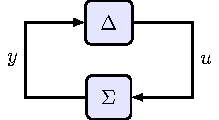
\includegraphics[valign=c]{sys-robust}
\end{center}

The dynamical system $\Sigma$ describes how the state $\xi_k$ of the system evolves in time as well as how the point $y_k$ at which the oracle is evaluated depends on the state and input of the system. The operator $\Delta$ evaluates the oracle at the point $y_k$ to produce the input $u_k$ to the system, which can be intepreted as an uncertainty over the functions $f\in\F$. This can be represented graphically as the system $\Sigma$ in feedback with the uncertainty $\Delta$, as is typical in robust control~\cite{ZDG}.

The closed-loop system is typically a nonlinear dynamical system due to the oracle. The main idea behind the analysis is to replace the oracle with inequalities that hold between its input and output.
%For instance, if $f$ is convex, then the inequality $(\df(y_2)-\df(y_1))^\tp (y_2-y_1) \geq 0$ holds for all $y_1,y_2\in\real^d$. Note that this condition involves the gradient evaluated at two points, such as two consecutive iterates of the algorithm.
% The more points along the trajectory of the algorithm to which we apply this inequality, the tighter the analysis. To obtain a sequence of points, we filter the input and output signals of the gradient with a filter $\psi(z) = (1,z^{-1},\ldots,z^{-\ell+1})$ for some integer $\ell$ so that the filtered signals are as follows:\\
% \[
%   \bmat{\y \\ \u} = \Psi\bmat{y \\ u} \qquad\text{where}\qquad
%   \y_t = \bmat{y_t \\ \vdots \\ y_{t-\ell+1}} \qquad\text{and}\qquad
%   \u_t = \bmat{u_t \\ \vdots \\ u_{t-\ell+1}}.
%   % \Psi(z) = \bmat{1 & z^{-1} & \ldots & z^{-\ell+1} & 0 & 0 & \ldots & 0 \\ 0 & 0 & \ldots & 0 & 1 & z^{-1} & \ldots & z^{-\ell+1}}^\tp
% \]
Consider applying a filter $\Psi$ to the input $y$ and output $u$ of the uncertainty. IQCs are then quadratic inequalities on the output of the filter that are known to hold for all possible uncertainties~\cite{iqc}. The uncertainty $\Delta$ can then be replaced by these constraints as follows:
\begin{center}
  \centering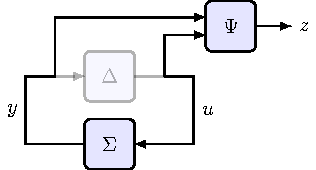
\includegraphics{iqc}
\end{center}
which simplifies to:
\begin{center}
  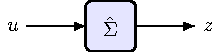
\includegraphics{sys-closed-loop}
\end{center}
subject to the IQC
\[
    0\leq\sum_{k=0}^{N-1} z_k^\tp M z_k.
\]
Here, $\hat\Sigma$ represents the closed-loop map from $u$ to $z$, which depends on both the system $\Sigma$ and filter $\Psi$. The analysis then reduces to studying the closed-loop system $\hat\Sigma$ subject to the IQCs on its output. If the system $\hat\Sigma$ has a certain convergence property whenever the IQC is satisfied, and the IQC holds for any uncertainty $\Delta$, then the convergence property must hold for the original feedback interconnection of $\Sigma$ with $\Delta$.

To illustrate the analysis, suppose the closed-loop system $\hat\Sigma$ is linear and time invariant with state-space representation $(\hat A,\hat B,\hat C,\hat D)$. If we can find a positive definite matrix $P\succ 0$ and scalar $\lambda\geq 0$ such that the linear matrix inequality (LMI)
\begin{multline*}
    \bmat{\hat A & \hat B}^\tp P \bmat{\hat A & \hat B} - \rho^2\bmat{I & 0}^\tp P \bmat{I & 0} \\ + \lambda\bmat{\hat C & \hat D}^\tp M \bmat{\hat C & \hat D} \preceq 0
\end{multline*}
holds, then the quadratic form $V(\hat\xi) = \hat\xi^\tp P \hat\xi$ is a Lyapunov function for the system, where $\hat\xi_k$ is the state of the closed-loop system $\hat\Sigma$. In particular, feasibility of this LMI certifies that the iterates converge linearly since
\[
  \|\hat\xi_k\|^2 \leq V(\hat\xi_k) \leq \rho^2 V(\hat\xi_{k-1}) \leq \ldots \leq \rho^{2k} V(\hat\xi_0).
\]
The first inequality is due to $P$ being positive definite while the remaining ones are due to the LMI.

\subsection{Relationship Between the Two Approaches}

The IQC and PEP approaches to automated algorithm analysis are related: they are \textit{dual} problems of each other~\cite{taylor2018lyapunov}. This insight has numerous benefits. For instance, IQCs can be derived directly from the interpolation conditions for a class of uncertainties, which provides a systematic method to construct IQCs as well as theoretical guarantees about the tightness of the constraints and the resulting analysis. Similar to the PEP approach, the IQC analysis extends in a straightforward manner to include \textit{function values}. When the uncertainty is the gradient of a function, $\Delta = \df$, we can include the function values $f(y_t)$ in the analysis to handle function classes that are defined by inequalities involving them, such as quadratic growth which is defined by the inequality $f(x) \geq \frac{\mu}{2} \|x\|^2$ for all $x$. In either case, the analysis consists of solving a convex semidefinite program for which efficient solvers~\cite{mosek,cosmo,scs} and modeling languages~\cite{yalmip,cvx1,cvx2} are readily available.

\section{Package Structure}

The package transforms the algorithm description into a mathematical optimization problem, which is then modeled in JuMP~\cite{JuMP,JuMP-review} and solved using an appropriate solver. The package is designed to be extensible, allowing users to add new types of algorithms and performance measures as needed.

\section{Examples}

\section{Conclusion}


% \vadjust{\vfill\pagebreak} % to balance the last page

\input{bib.tex}

\end{document}
